\subsection{NASA single-tooth force}
\label{sec:nasa-tooth-force}

We compare the single-tooth normal force against the solid experimental
traces in Fig.~7 of \href{https://ntrs.nasa.gov/citations/19910013253}{NASA TM-103232}.
Both solvers use the reconstructed 28/28-tooth fixture, the published SI
inertias and shaft stiffnesses, and identical effective contact parameters.
The 2,000 rpm, 33.73 N\,m condition sets the equivalent normal stiffness
and damping. The two 6,000 rpm conditions use those frozen parameters.
Complete simulated engagements are averaged at the same actual driven-tooth
roll angles. The scored range ends at \(29.5^\circ\) and starts at
\(12^\circ\) for 7(a,c) and \(12.625^\circ\) for 7(d).

Figure~\ref{fig:nasa-tooth-force} shows substantial agreement in the
force envelope for 7(a,d). In 7(c) the simulation underestimates the first
crest and overestimates the force near the trailing transition. The
figure and table present three conditions. In the fourth condition,
4,000 rpm and 11.48 N\,m, the experiment shows tooth separation while
both models retain positive load in the center of that interval.
The full four-condition comparison and the excluded condition's metrics
are available in the experiment archive.

\begin{table}[!htbp]
\centering\small
\caption{Single-tooth force errors for the three displayed NASA conditions.
RMSE uses the published roll-angle origin and a \(0.125^\circ\) grid.}
\label{tab:nasa-tooth-force}
\begin{tabular}{lrrrrl}
\toprule
Panel & rpm & Torque (N\,m) & B-rep RMSE (N) & BVH RMSE (N) & Role \\
\midrule
\NasaSelectedRows
\bottomrule
\end{tabular}
\end{table}

\begin{figure}[!htbp]
\centering
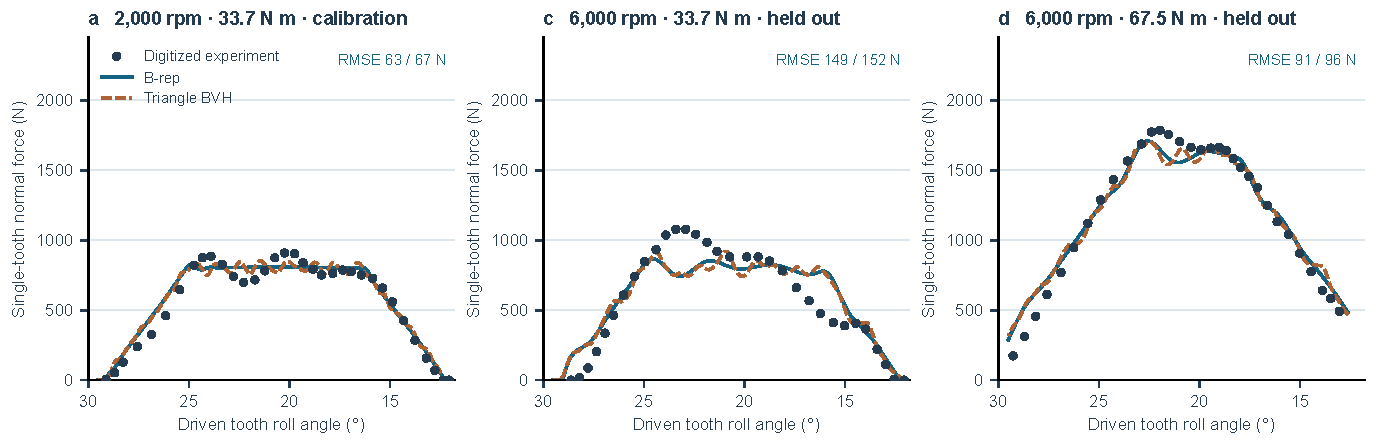
\includegraphics[width=\linewidth]{../results/gears/experimental/figures/nasa-single-tooth-selected.pdf}
\caption{Single-tooth force for NASA Fig.~7(a,c,d). Markers represent the
digitized measurement, and the lines represent simulations with B-rep
geometry and a triangle BVH.}
\label{fig:nasa-tooth-force}
\end{figure}
